\documentclass{article}
\usepackage[utf8]{inputenc}
\usepackage{lmodern}
\usepackage{blindtext}
\usepackage{amsmath}
\usepackage[a4paper, inner=1.7cm, outer=2.7cm, top=3cm, bottom=3cm, bindingoffset=1.2cm]{geometry}
\usepackage{tcolorbox}
\usepackage{graphicx}
\usepackage{wrapfig}
\usepackage{makecell}
\usepackage{boldline}
\usepackage{float}
\usepackage{tabularx}
\usepackage[table]{colortbl}
\usepackage[english]{babel}
\usepackage{amsthm}
\usepackage{hyperref}

\newtheorem*{invariant}{Invariant}

\renewcommand\theadalign{bc}
\renewcommand\theadfont{\bfseries}
\renewcommand\theadgape{\Gape[4pt]}
\renewcommand\cellgape{\Gape[4pt]}

\begin{document}

\title{\textbf{LUSDChickenBonds Shifting Profitability}}
\author{Daniel Simon}
\date{June 15, 2021}

\maketitle

\section{Introduction}
The idea behind the shifting functions of LUSDChickenBonds is to allow the ``owned" LUSD to act as a moving mass: it can serve as liquidity (in the Curve LUSD-3CRV metapool) when liquidity is needed the most, or provide stability through the Stability Pool when less liquidity is needed. Because of the permissionless nature of the functions, it is crucial that we ensure they can't be used in a way that would result in a loss to the protocol.

\subsection{Intuition}
Let's disregard fees for a second. Our intuition is that single-sidedly depositing LUSD while the pool is light on LUSD, and single-sidedly withdrawing LUSD while the pool is heavy on LUSD are profitable actions under the assumption that LUSD should eventually return to \$1.

\subsection{Informal reasoning}

By adding liquidity to a pool (single-sided or not) we are given LP tokens in return, entitling us to a pro-rata share of the pool's reserves of each coin. This means that depositing single-sidedly (into a pool of 2 coins) involves implicitly swapping a portion of our input coin into the other coin. Similarly, withdrawing single-sidedly involves swapping one side of our pro-rata share of the pool into the other coin.

In the case of the LUSD-3CRV metapool: when the pool is light on LUSD, the spot price of LUSD in the pool will be more than \$1. Making a single-sided LUSD deposit that moves the pool closer to being balanced amounts to selling part of the LUSD at a favorable rate (when it's ``expensive"). On the other hand: when the pool is heavy on LUSD, its spot price will be less than \$1. Withdrawing LUSD single-sidedly in this state amounts to buying LUSD at a favorable rate (when it's ``cheap").

\subsection{With fees}

The existence of fees somewhat complicates things by reducing the rate at which our coins are swapped during single-sided liquidity changes (or non-proportional in general). In practice, we expect this to make balance-improving single-sided liquidity changes a net loss if the pool is already close to being balanced, such that the price of LUSD is roughly in the range of $1 \pm fee$.

Our approach is to run simulations across a sweep of ``A" factors and spot prices to find out more precisely where the boundaries of profitability lie. Based on our findings we will choose spot price thresholds for depositing and withdrawing that ensure profitability under any A that might realistically be set by governance.

\section{StableSwap Properties}

First we introduce a couple of useful properties of StableSwap, which we will later use to show that the results of our simulations can be scaled to any pool size. We've demonstrated that the properties hold through the use of randomized testing, but we expect they could be proven mathematically.

Let's suppose we have the following functions (partially) implementing the StableSwap invariant for the 2-coin case, where $x$ and $y$ are the pool's reserves of coin 1 and 2:

\begin{itemize}
\item $D(x, y)$: pool's invariant ``D" as a function of the reserves
\item $dydx(x, y)$: the spot price $-dy/dx$ between coins 1 and 2
\item $x_d(x, y, \Delta{x}, \Delta{y})$: pool's reserve of coin 1 after a deposit of $\Delta{x}$, $\Delta{y}$
\item $y_d(x, y, \Delta{x}, \Delta{y})$: pool's reserve of coin 2 after a deposit of $\Delta{x}$, $\Delta{y}$
\item $\Delta{t}_d/t(x, y, \Delta{x}, \Delta{y})$: LP shares minted in exchange for a deposit of $\Delta{x}$, $\Delta{y}$, as a fraction of the (old) total supply t, such that the new total supply is $t' = t(1 + \Delta{t}_d/t)$
\item $x_{w1}(x, y, \Delta{t}/t)$: pool's reserve of coin 1 after a single-sided withdrawal of coin 1 that burns fraction $\Delta{t}/t$ of the (old) total supply of LP shares
\item $y_{w1}(x, y, \Delta{t}/t)$: pool's reserve of coin 2 after a single-sided withdrawal of coin 1 that burns fraction $\Delta{t}/t$ of the (old) total supply of LP shares
\item $\Delta{x}_{w1}(x, y, \Delta{t}/t)$: the amount of coin 1 received when burning fraction $\Delta{t}/t$ of the (old) total supply to withdraw single-sidedly
\end{itemize}

All functions implicitly depend on the A, fee and $admin\_fee$ parameters, except for $D()$ and $dydx()$, which don't depend on fee or $admin\_fee$.

\subsection{Property \#1: D homogeneity}

The function $D()$ is positively homogeneous of degree 1, i.e. for $s > 0$:
\[
D(sx, sy) = sD(x,y)
\]

Test:
\url{https://github.com/liquity/ChickenBond/blob/b344f8d25ad6bade72092e53c505a8ea5f81b129/tools/sand-buckets/test/pool-prop.test.ts#L84-L94}

\subsection{Property \#2: spot price homogeneity}

The function $dydx()$ is positively homogeneous of degree 0:
\[
dydx(sx, sy) = dydx(x, y)
\]

Test:
\url{https://github.com/liquity/ChickenBond/blob/b344f8d25ad6bade72092e53c505a8ea5f81b129/tools/sand-buckets/test/pool-prop.test.ts#L96-L130}

\subsection{Property \#3: spot price monotonicity}

Given property \#2, we can express the spot price as a function of only the ratio $y/x$:
\[
dydx(x, y) = dydx(x/x, y/x) = dydx(1, y/x) = g(y/x)
\]

We find that the function $g()$ is strictly monotone, which makes it injective. In other words, there is a unique ratio $y/x$ between the pool's reserves for each spot price.

Test:
\url{https://github.com/liquity/ChickenBond/blob/b344f8d25ad6bade72092e53c505a8ea5f81b129/tools/sand-buckets/test/pool-prop.test.ts#L132-L168}

\subsection{Property \#4: deposit homogeneity}

The functions $x_d()$, $y_d()$ are positively homogeneous of degree 1:
\[
x_d(sx, sy, s\Delta{x}, s\Delta{y}) = s x_d(x, y, \Delta{x}, \Delta{y})
\]

\[
y_d(sx, sy, s\Delta{x}, s\Delta{y}) = s y_d(x, y, \Delta{x}, \Delta{y})
\]

The function $\Delta{t}_d()$ is positively homogeneous of degree 0:
\[
\Delta{t}_d/t(sx, sy, s\Delta{x}, s\Delta{y}) = \Delta{t}_d/t(x, y, \Delta{x}, \Delta{y})
\]

Test:
\url{https://github.com/liquity/ChickenBond/blob/b344f8d25ad6bade72092e53c505a8ea5f81b129/tools/sand-buckets/test/pool-prop.test.ts#L212-L241}

\subsection{Property \#5: one-coin withdrawal homogeneity}

The functions $x_{w1}()$, $y_{w1}()$ and $\Delta{x}_{w1}()$ are positively homogeneous of degree 1 in the variables $x$, $y$:
\[
x_{w1}(sx, sy, \Delta{t}/t) = sx_{w1}(x, y, \Delta{t}/t)
y_{w1}(sx, sy, \Delta{t}/t) = sy_{w1}(x, y, \Delta{t}/t)
\Delta{x}_{w1}(sx, sy, \Delta{t}/t) = s \Delta{x}_{w1}(x, y, \Delta{t}/t)
\]

Test:
\url{https://github.com/liquity/ChickenBond/blob/b344f8d25ad6bade72092e53c505a8ea5f81b129/tools/sand-buckets/test/pool-prop.test.ts#L243-L267}

\section{Simulation}

\subsection{Marginal profit}

Our approach is to simulate single-sided deposits/withdrawals of practically infinitesimal size over a wide range of spot prices and a selection of ``A" factors between 10-5000.

\subsubsection{Definition for deposits}

Let's define the following function for notational convenience, which is a shorthand for the pool's new invariant ``D" after single-sidedly depositing $\Delta{x}$ of coin 1 (in our case: LUSD) into $x$, $y$:
\[
D_{d1}(x, y, \Delta{x}) = D(x_d(x, y, \Delta{x}, 0), y_d(x, y, \Delta{x}, 0))
\]

We are assuming that the LP shares we receive are worth their virtual price in dollars. The definition of virtual price $v$ when $t$ is the total supply of LP shares:
\[
v = D / t
\]

We get the value of shares received for depositing $\Delta{x}$ into $x$, $y$ by multiplying the number of shares by the new virtual price after the deposit:
\[
\begin{split}
  v_{d1}(x, y, \Delta{x}) &= (t * \Delta{t}_d/t(x, y, \Delta{x}, 0)) * (D_{d1}(x, y, \Delta{x}) / (t * (1 + \Delta{t}_d/t(x, y, \Delta{x}, 0)))) \\
  &= \Delta{t}_d/t(x, y, \Delta{x}, 0) * D_{d1}(x, y, \Delta{x}) / (1 + \Delta{t}_d/t(x, y, \Delta{x}, 0)) \\
  &= D_{d1}(x, y, \Delta{x}) * (1 - 1 / \Delta{t}_d/t(x, y, \Delta{x}, 0))
\end{split}
\]

We assume that the true price of LUSD is \$1 irrespective of the current Curve spot price, and define marginal profit of a single-sided deposit as:
\[
pmd(x, y, \Delta{x}) = (v_{d1}(x, y, \Delta{x}) - \Delta{x}) / \Delta{x} = v_{d1}(x, y, \Delta{x}) / \Delta{x} - 1,
\]

in which $\Delta{x}$ should be small enough not to introduce significant slippage.

We aim to show that this definition of marginal profit is the same for any pool state having the same initial price and relative change in $x$, in other words: that $pmd()$ is scale invariant:
\[
pmd(sx, sy, s\Delta{x}) \stackrel{?}{=} pmd(x, y, \Delta{x})
\]

Substituting into the body of $pmd(sx, sy, s\Delta{x})$:
\[
\begin{split}
  v_{d1}(sx, sy, s\Delta{x}) / s\Delta{x} - 1 &= D_{d1}(sx, sy, s\Delta{x}) * (1 - 1 / \Delta{t}_d/t(sx, sy, s\Delta{x}, 0)) / s\Delta{x} - 1 \\
  &= D(x_d(sx, sy, s\Delta{x}, 0), y_d(sx, sy, s\Delta{x}, 0)) * (1 - 1 / \Delta{t}_d/t(sx, sy, s\Delta{x}, 0)) / s\Delta{x} - 1
\end{split}
\]

Using property \#4 for $\Delta{t}_d/t()$, $x_d()$ and $y_d()$:
\[
D(sx_d(x, y, \Delta{x}, 0), sy_d(x, y, \Delta{x}, 0)) * (1 - 1 / \Delta{t}_d/t(x, y, \Delta{x}, 0)) / s\Delta{x} - 1
\]

Using property \#1 for $D()$ and simplifying:
\[
\begin{split}
  &sD(x_d(x, y, \Delta{x}, 0), y_d(x, y, \Delta{x}, 0)) * (1 - 1 / \Delta{t}_d/t(x, y, \Delta{x}, 0)) / s\Delta{x} - 1 \\
  &= D(x_d(x, y, \Delta{x}, 0), y_d(x, y, \Delta{x}, 0)) * (1 - 1 / \Delta{t}_d/t(x, y, \Delta{x}, 0)) / \Delta{x} - 1
\end{split}
\]

Replacing subexpression with functions we get the expression we're looking for:
\[
D_{d1}(x, y, \Delta{x}) * (1 - 1 / \Delta{t}_d/t(x, y, \Delta{x}, 0)) / \Delta{x} - 1 = v_{d1}(x, y, \Delta{x}) / \Delta{x} - 1 = pmd(x, y, \Delta{x})
\]

Therefore, the marginal profit for single-sided deposit at a given spot price is independent of pool size.

\subsubsection{Definition for withdrawals}

We once again assume that the LP tokens we burn are worth their virtual price in dollars, and define the value of burnt shares as:
\[
v_b(x, y, \Delta{t}/t) = (t * \Delta{t}/t) * (D(x, y) / t) = \Delta{t}/t * D(x, y)
\]

Assuming LUSD is \$1, we define marginal profit of single-sided withdrawal as:
\[
pmw(x, y, \Delta{t}/t) = (\Delta{x}_{w1}(x, y, \Delta{t}/t) - v_b(x, y, \Delta{t}/t)) / v_b(x, y, \Delta{t}/t) =
  = \Delta{x}_{w1}(x, y, \Delta{t}/t) / v_b(x, y, \Delta{t}/t) - 1,
\]

in which $\Delta{t}$ should be small enough not to introduce significant slippage.

It can be shown that this is also scale invariant in $x$ and $y$:

\[
pmw(sx, sy, \Delta{t}/t) = \Delta{x}_{w1}(sx, sy, \Delta{t}/t) / v_b(sx, sy, \Delta{t}/t) - 1 =
  = s\Delta{x}_{w1}(x, y, \Delta{t}/t) / bD(sx, sy) - 1 = s\Delta{x}_{w1}(x, y, \Delta{t}/t) / sbD(x, y) - 1 =
  = \Delta{x}_{w1}(x, y, \Delta{t}/t) / bD(x, y) - 1 = \Delta{x}_{w1}(x, y, \Delta{t}/t) / v_b(x, y, \Delta{t}/t) - 1 =
  = pmw(x, y, \Delta{t}/t)
\]

Therefore, the marginal profit for single-sided withdrawal at a given spot price is independent of pool size.

\subsubsection{Implementation}

We choose some arbitrary (large) value $D_0$ for the pool invariant ``D", and for each combination of ($dydx_i$, $A_j$) we exploit property \#3 to find the unique pair $(x,y)$ for which $D(x,y)=D0$ and $dydxA=A_j(x,y)=dydx_i$ by binary search. We then evaluate $pmd()$ and $pmw()$ using relatively small values for $\Delta{x}$ and $\Delta{t}/t$ ($D/10^9$ in the case of $\Delta{x}$ and $1/10^9$ for $\Delta{t}/t$).

Code:
\url{https://github.com/liquity/ChickenBond/blob/b344f8d25ad6bade72092e53c505a8ea5f81b129/tools/sand-buckets/src/sheets/marginal-deposit.ts}
\url{https://github.com/liquity/ChickenBond/blob/b344f8d25ad6bade72092e53c505a8ea5f81b129/tools/sand-buckets/src/sheets/marginal-withdrawal.ts}

\subsubsection{Results}

We see that depositing becomes profitable around the $dy/dx = 1+fee$ mark as expected, but that the exact point depends on the variable ``A" factor of the pool (adjustable by governance) and is shifted slightly towards higher $dy/dx$ (more imbalance) at higher A's:

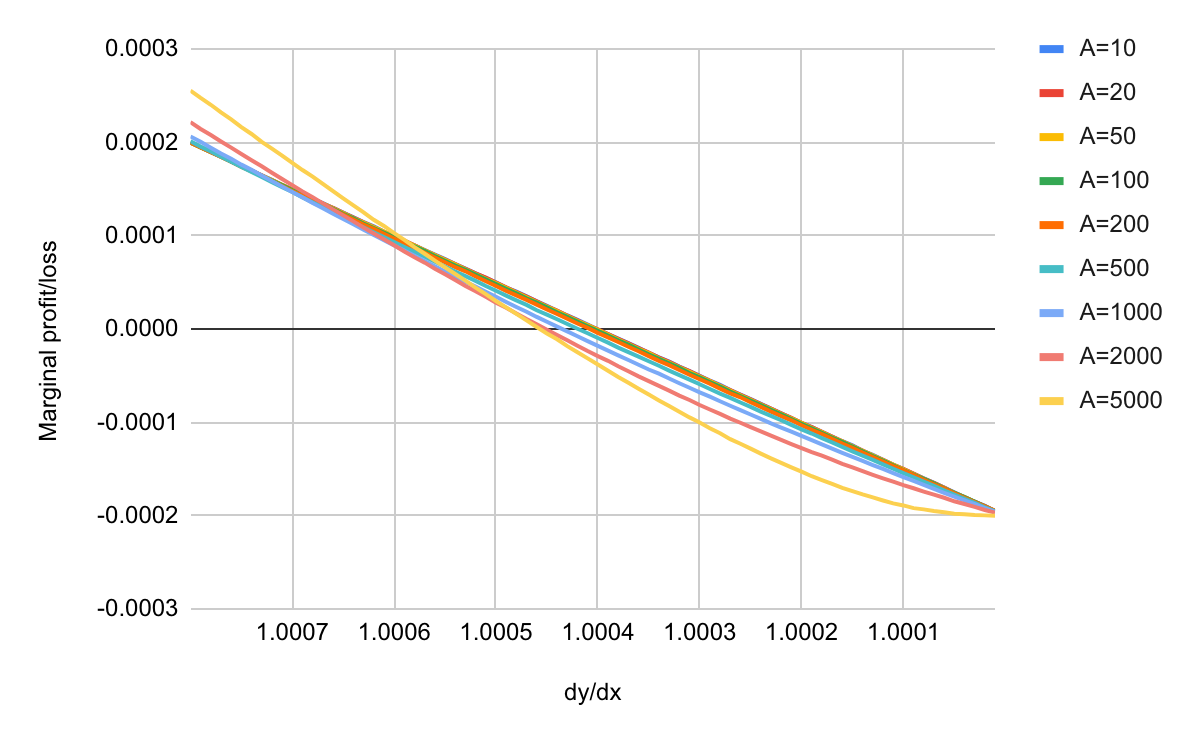
\includegraphics[width=\linewidth]{./LUSDChickenBonds_Shifting_Profitability_1.png}

Therefore it makes sense to choose a threshold slightly higher than 1+fee for allowing deposits (i.e. shifting SP => Curve), e.g. 1.0005.

We further find that depositing only becomes more profitable as dy/dx increases into absurd range:

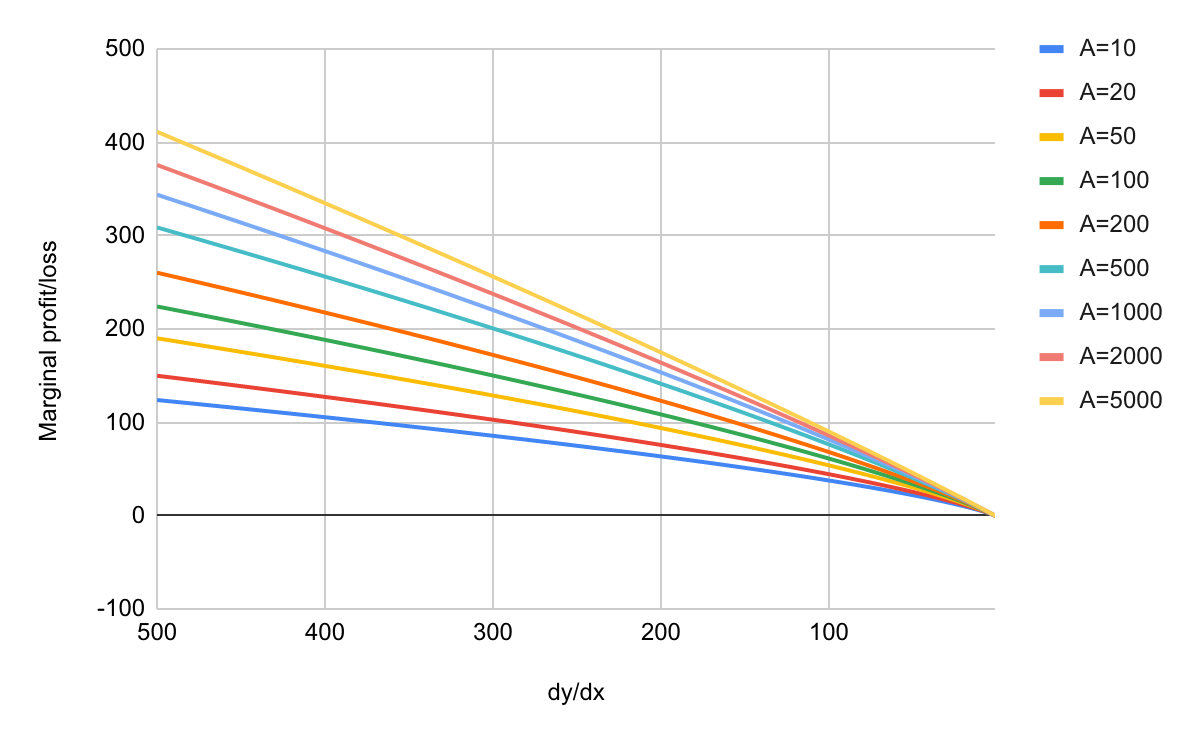
\includegraphics[width=\linewidth]{./LUSDChickenBonds_Shifting_Profitability_2.png}

In the case of withdrawal, we see that it also becomes profitable around dx/dy = 1+fee, but the exact point is shifted in the other direction, towards lower dx/dy (less imbalance):

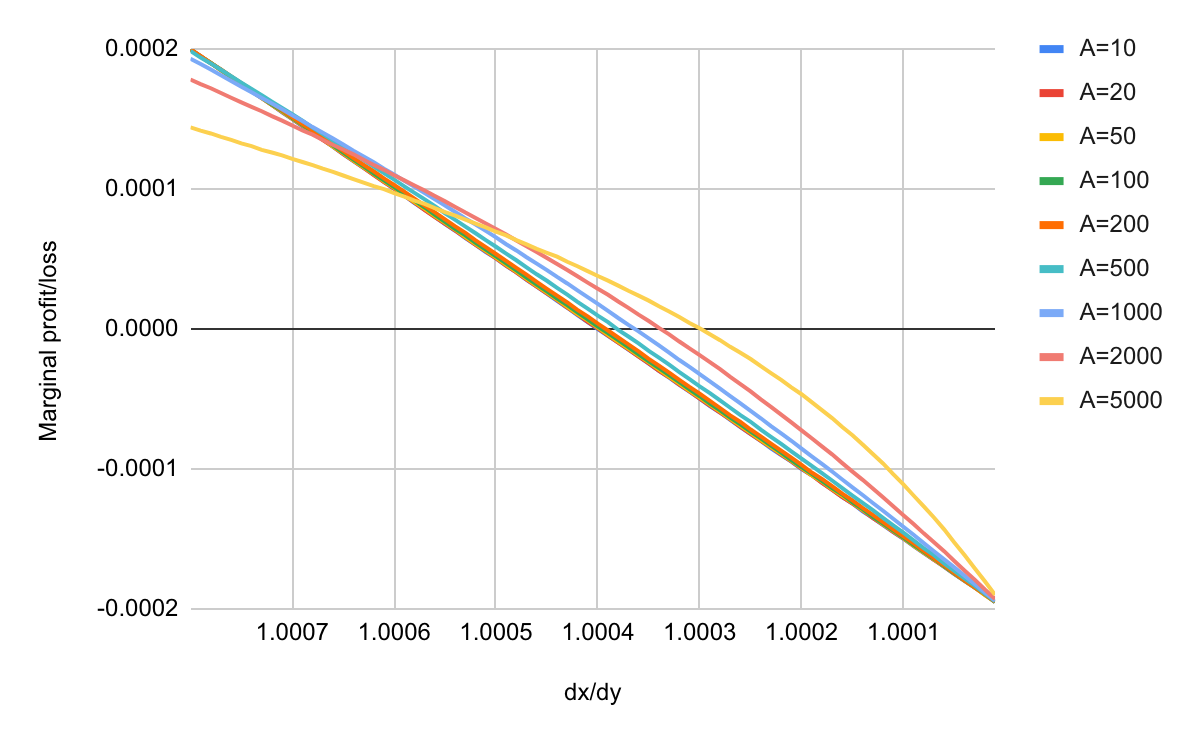
\includegraphics[width=\linewidth]{./LUSDChickenBonds_Shifting_Profitability_3.png}

Just as in the case of deposits, withdrawal only becomes more profitable at absurdly high dx/dy:

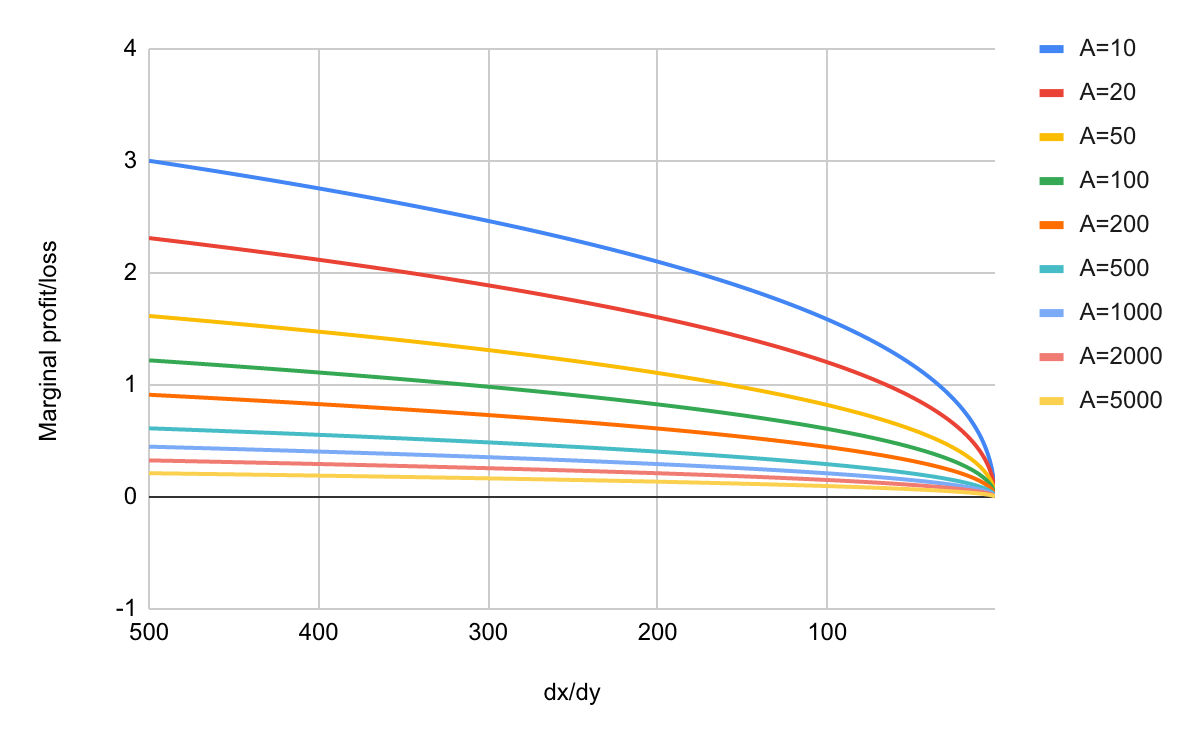
\includegraphics[width=\linewidth]{./LUSDChickenBonds_Shifting_Profitability_4.png}

\subsection{ROI of maximal shifts}

We call a shift (either SP => Curve or Curve => SP) starting from a particular spot price maximal, if it ends at our chosen threshold for allowing a shift in that particular direction. In other words, any attempt to shift a higher amount would not be allowed due to our final check on the spot price.

It is interesting to note that the ROI of a maximal shift is actually the lowest ROI that can be achieved by a shift, and submaximal shifts are actually more profitable in terms of ROI. This comes from the fact that marginal profit decreases the closer the spot price is to perfect balance.

Code:
\url{https://github.com/liquity/ChickenBond/blob/b344f8d25ad6bade72092e53c505a8ea5f81b129/tools/sand-buckets/src/sheets/walled-deposit.ts}
\url{https://github.com/liquity/ChickenBond/blob/b344f8d25ad6bade72092e53c505a8ea5f81b129/tools/sand-buckets/src/sheets/walled-withdrawal.ts}

\subsubsection{Deposit (to dy/dx = 1.0005)}

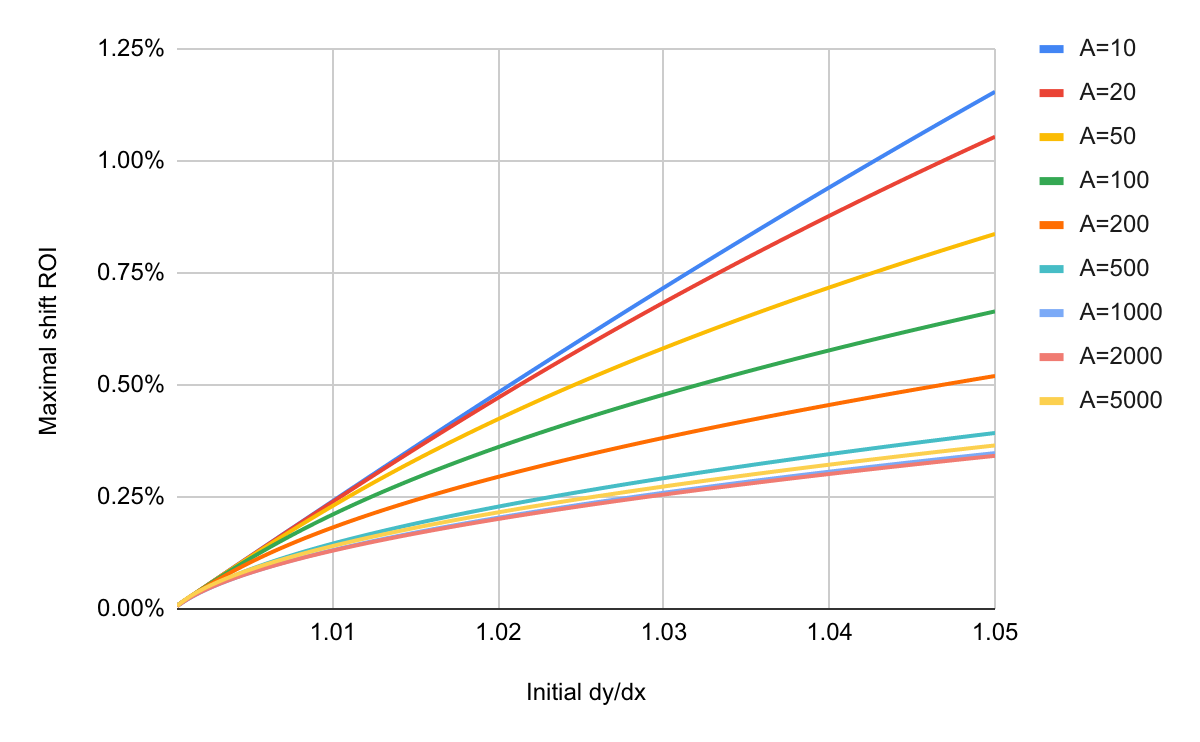
\includegraphics[width=\linewidth]{./LUSDChickenBonds_Shifting_Profitability_5.png}

\subsubsection{Withdrawal (to dx/dy = 1.0004)}

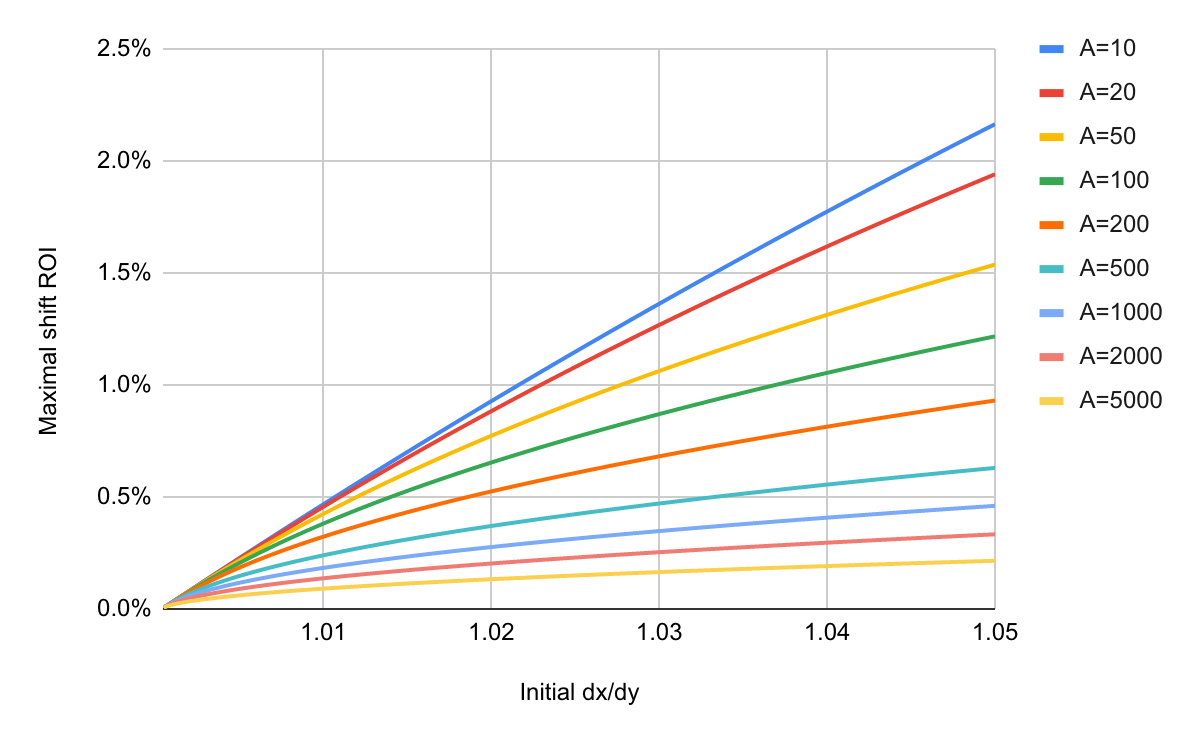
\includegraphics[width=\linewidth]{./LUSDChickenBonds_Shifting_Profitability_6.png}

\subsection{Spreadsheets}

Link:
\url{https://docs.google.com/spreadsheets/d/1FKwuPD5N6RPTQtYzTWb6NsoEYtpCCZKheYxMplKvD4w/edit#gid=971124440}


\end{document}
